\chapter{Einlesen der MIDI-Files}


\begin{enumerate}[a)]
% a)
\item
Siehe MATLAB-Code:
\begin{itemize}
\item
main.m
\end{itemize}

\item
Siehe MATLAB-Code:
\begin{itemize}
\item
createNotes.m
\end{itemize}
\item
\begin{figure}
  \centering
      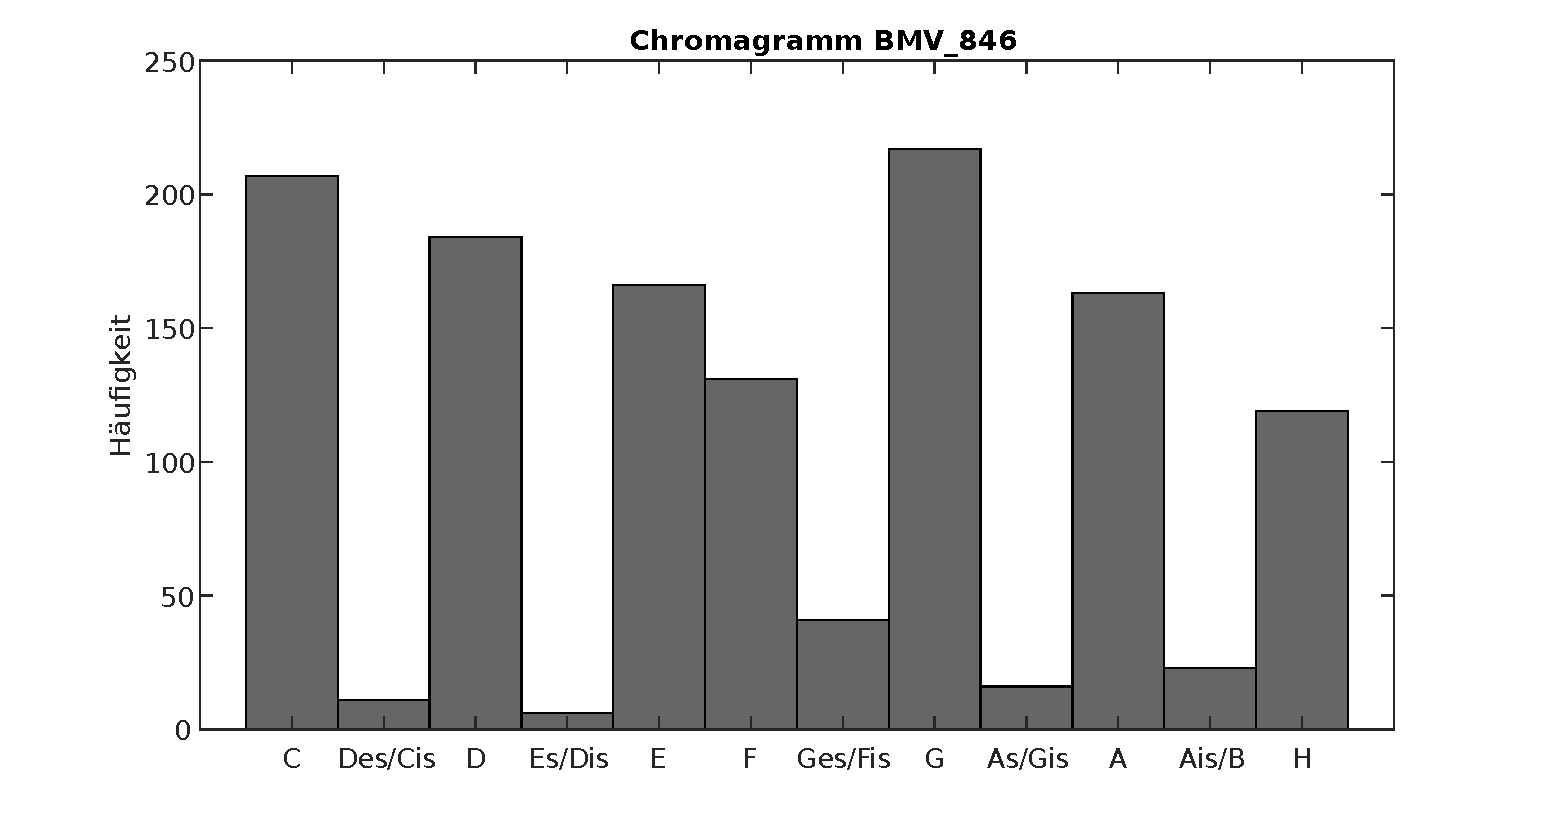
\includegraphics[width=0.9\textwidth]{Figures/Chromagram1}
      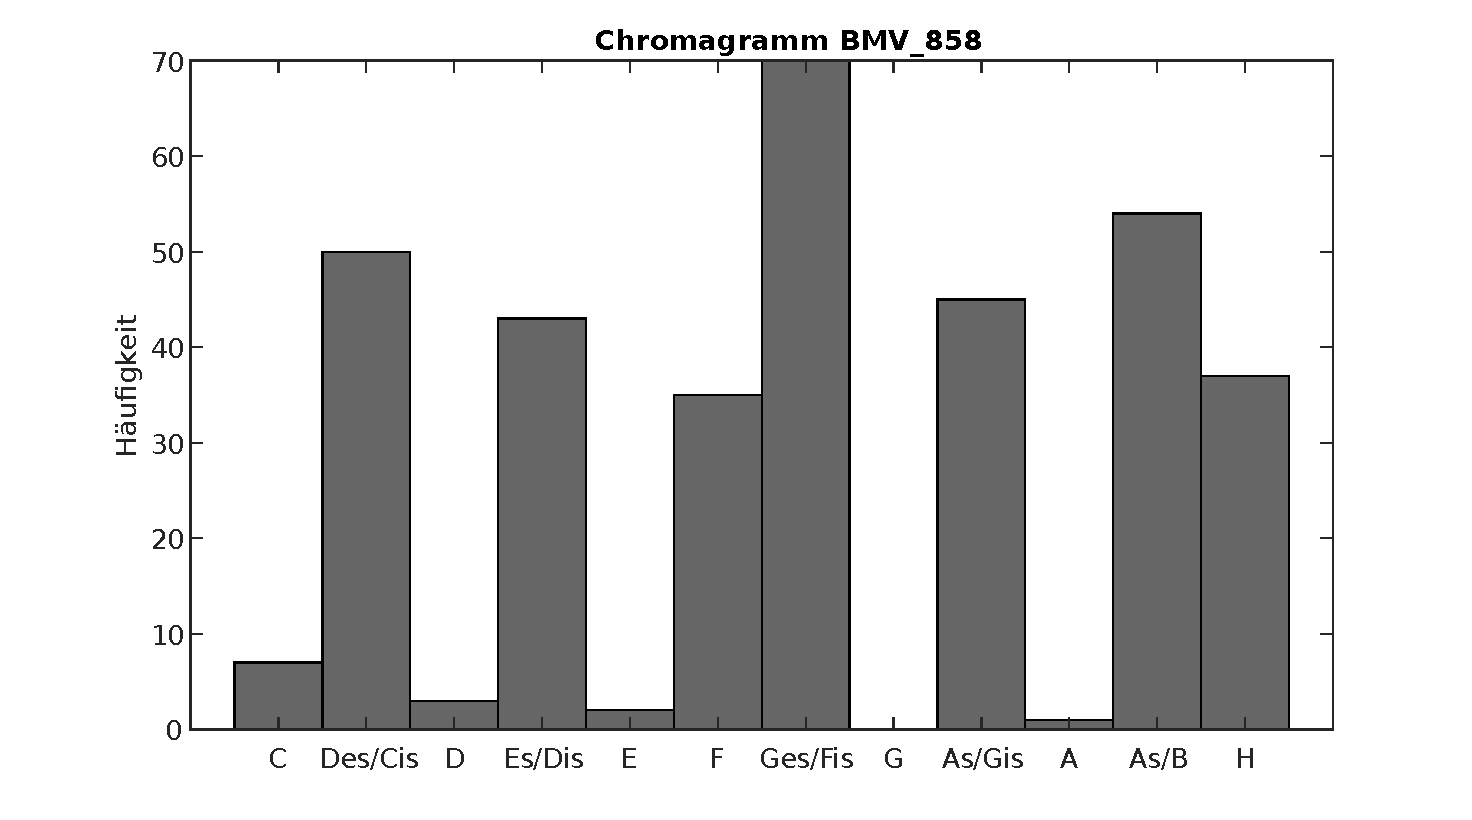
\includegraphics[width=0.9\textwidth]{Figures/Chromagram2}
 \caption{Chromagramm der Notenhäufigkeiten in den beiden Stücken}
	\label{fig:chr}
\end{figure}
Anhand der Notenhäufigkeiten, wie in Abbildung \ref{fig:chr} zu sehen, lassen sich die Ganzton-Halbtonstrukturen und somit die Tonarten der beiden Stücke ablesen:\\
Das Stück aus \textit{BWV\_846.mid} steht in C-Dur. Was zudem dafür spricht, dass es nicht in der parallen Molltonart steht, ist das häufige Vorkommen vom Grundton C und der Quinte G.\\
Das Stück \textit{BWV\_858.mid} steht in Ges-Dur. Dafür spricht wiederum die Ganzton-Halbtonstruktur sowie das häufige Vorkommen des Grundtons Ges, der Terz As und der Quinte Des.
\end{enumerate}

